\section{Internet-scale analysis}
\label{sec:internet-scale}

We explore how effective \name attacks might be in
practice by modeling the activity of Tor users, emulating the
corresponding Tor path selection of these users, and inferring  the
prevalence of AS-level adversaries who have the ability to
mount the attacks that we described in the preceding sections.

\subsection{Approach}

Figure~\ref{fig:simulations} summarizes our approach, which we detail in
the next section. We model the activity of Tor users and simulate
corresponding Tor path selection using TorPS~\cite{TorPS}.  TorPS
returns guard and exit relays, which we then feed as input---together
with source ASes and destination addresses---into our framework that
runs traceroutes from RIPE Atlas nodes.  The rest of this section
describes our approach in detail.

\subsubsection{Attack model}

\begin{figure}[t]
	\centering
	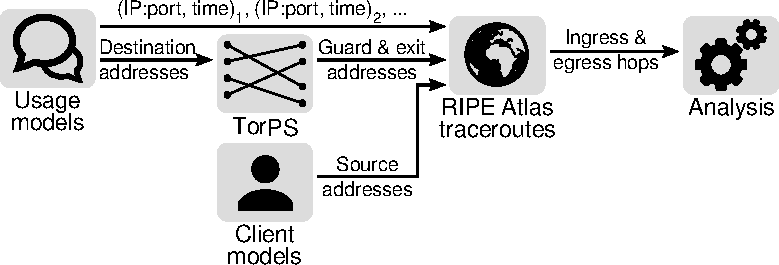
\includegraphics[width=\linewidth]{figures/simulations.pdf}
	\caption{The relation among our simulation components.  Our goal is to
	determine the ASes a Tor user's traffic traverses into and out of the Tor
	network.  Duplicate ASes on both sides can deanonymize streams.}
	\label{fig:simulations}
\end{figure}

We assume that an AS that can see traffic entering the Tor network and
and can see DNS traffic exiting the Tor network at the other end can use
this information in order to deanonymize the entering traffic.  Here we
seek to measure the chances an AS will be in this favorable position to
carry out such an attack.

A Tor exit can perform DNS resolution in two ways: running a name server
locally; relying on a third-party name server, such as its ISP's name
server or a public DNS name server such as Google's open public DNS
resolver ({\tt 8.8.8.8}).  In the case of Tor
exits that perform local DNS resolution a good position for an attacker
might be both (1)~anywhere on the AS path between a Tor client and a Tor
guard; and (2)~anywhere on the path between a Tor exit and any of the
name servers the exit has to communicate with to resolve the name.
These name servers include the root name server, the TLD servers, and
the second-level servers.  The ASes along the path from the exit relay
to the name servers will be able to see the domain names that the exit
relay is querying.

For Tor exits that rely on a third-party for DNS resolution, an
adversary might be on the path between a Tor client and a
Tor guard and on the path between a Tor exit and the third-party name
server.  In additionx, the DNS queries will look like they are coming
from the IP address of the name server and not the IP address of the
exit relay.

\subsubsection{Simulating Tor user activity: TorPS}

To measure the likelihood that an AS can be in a position to perform a
\name attack, we use TorPS, the Tor Path Simulator, which
mimics how the Tor client software constructs circuits.
TorPS thus provides realistic combinations of guards and exits based on the state of the 
Tor network at a given time. TorPS is based on Tor version \xxx{X}. For each sample, it uses 
one guard which expires after 270 days. We use TorPS to emulate the behavior of a Tor 
client for the month of March 2016.  As in previous work, we perform
100,000 iterations (\ie, guard-exit pairs).
 For our simulation, we had each sample 
visit {\tt domain.com}\footnote{We redacted the real domain to anonymize our
submission.}---a website under our control---once per hour for all
of March 2016.  Thus, each guard-exit pair had 744 opportunites to be
compromised (this assumes that the circuit changes for every visit to
{\tt domain.com}). 
% It is much better to use a tool like TorPS in order to
%measure these chances instead of just using all permutations of guard and exits.

The paragraph changes a lot: Made our own model based off of UGR ``typical'' model.  
The sample user visits nine websites during the course of his day: mail.google.com, 
twitter.com, calendar.google.com, instagram.com, startpage.com, ixquick.com, docs.google.com, 
facebook.com, and google.com.  \fixme{Should we mention the fixes we made to TorPS? Should we mention 
the problem we found with their user models? YES.}

In this analysis, we ignore caching of any type, so our results are overly 
pessimistic in this respect. \fixme{Mention that these results apply
  only to what we had data for: about half.}


\subsubsection{Inferring AS-level paths: traceroute + {\tt pyasn}}


% - 197 out of all 377 (52%) Tor exit ASes have Atlas probes.
% - 220 out of all 434 (51%) Tor guard ASes have Atlas probes.

% - Atlas ASes cover 57.53% of Tor exit bandwidth.
% - Atlas ASes cover 73.59% of Tor guard bandwidth.

\begin{table}[t]
	\caption{The coverage of RIPE Atlas nodes that are colocated with Tor guard and exit
	relays.}
	\label{tab:atlas-coverage}
	\centering
	\begin{tabular}{l|r r}
	\toprule
	\textbf{Atlas probe coverage} & \textbf{Tor guard ASes} & \textbf{Tor exit ASes} \\
	\midrule
	By bandwidth & 73.59\% & 57.53\% \\
	By number & 50.69\% & 52.25\% \\
	\bottomrule
	\end{tabular}
\end{table}


The Internet-wide experiment requires inferring the AS-level paths from
each exit relay to each destination. We decided against the (more
commonly applied) AS path inference because Juen \ea showed that it can
be quite inaccurate~\cite{Juen2015a}.  Using traceroute can yield more
accurate paths.  Measuring traceroutes from client to guard notes is
straightforward: we simply select a probe in a client AS and perform
traceroutes to each respective guard. \fixme{Mention why we picked AS
  6128 as our client AS.}  

Measuring traceroutes from exit relay to destination is far more
difficult because Tor does not impleement a mechanism to facilitate
traceroute~\cite{Murdoch2007a}. One approach, used in previous
work~\cite{Juen2015a}, is to ask relay operators to perform traceroutes.
Unfortunately, this approach only yielded traceroutes from relays
representing 26\% of exit bandwidth.  Instead, we observe that RIPE
Atlas~\cite{atlas} has probes in many ASes that have Tor exit relays.
We used this insight to design a measurement experiment to run
traceroutes from RIPE Atlas probes that were located in the same ASes as
Tor exits, to each of the destinations in question.  As shown in
Table~\ref{tab:atlas-coverage}, for a day in May 2016, we found that
RIPE Atlas had probes in 52\% of ASes that contain Tor exit relays.  We
found that RIPE Atlas has probes in 51\% of ASes that contain Tor guard
relays.  More importantly, we found that Atlas ASes cover 58\% of Tor
exit \textit{bandwidth} and 74\% of Tor guard bandwidth. (This statistic
is important because Tor relay usage is not evenly split among all of
the relays.) We considered using PlanetLab to initiate traceroutes, but
unfortunately most PlanetLab nodes are located in research and education
networks~\cite{banerjee2004interdomain} and are thus not well-suited for
performing these types of measurements.

Given these traceroutes, we mapped each IP address in every traceroute
to a corresponding AS.  The Python {\tt pyasn} module relies on BGP
routing tables to perform these mappings; by using a routing table that
coincides with the time when we performed our traceroutes, we can obtain
accurate AS-level mappings.  (This method of course is subject to
inaccuracies in the event of BGP route hijacks or leaks, but we expect
those events to be relatively unlikely for the time period and IP
prefixes that we are concerned with.)

The traceroutes are from July 2016, and we applied these in our analysis of Tor 
in March 2016.  \xxx{don't understand what ``analysis of Tor in March
  2016'' means.  What's the Tor trace corresponding to this?}



\subsection{Results}

Describe the four scenarios in the graph here: 1) ISPs, 2) Google, 3) Local, and 
4) Status Quo.

%Traditional: ``Traditional'' represents the paths between all exit ASes that RIPE Atlas 
%has coverage for and domain.com. That is, this measurement doesn't take DNS into account 
%at all, as has been traditionally done.
ISPs: ``ISPs'' represents what would happen if all exit relays used their ISPs' DNS name 
servers.  We choose to represent this by saying that the name server is in the same AS as the 
exit relay.

Google (8.8.8.8): ``Google'' represents what would happen if all exit relays used 
Google's public DNS server for resolution. We ran traceroutes from probes in all the exit 
ASes that RIPE Atlas had coverage for to 8.8.8.8.

Local: ``Local'' represents what would happen if all exit relays ran their own name 
servers locally (e.g., the use of unbound) on their own machines. In order to figure out 
what ASes would be traversed on the way to resolve domain.com. In order to figure out the 
DNS delegation path, we use the command line option \texttt{+trace} of the
command line tool dig. Assuming no caching and assuming 
iterative resolution, for domain.com the name server will have to visit three name servers:
a root name server, a top level domain name server, and a second-level domain name server. 

Status Quo: ``Status Quo'' represents to the best of our ability the type of name resolution 
that exit relays perform, whether that be their own or the use of 3rd-party name servers, 
which again includes public DNS name servers and their ISPs' name servers. To figure this 
out, we used the exitmap tool, our own website, and our own authoritative name server 
in order to figure out the IP addresses of the name servers that the exit relays were 
using. We then performed traceroutes from the exit ASes to the appropriate IP addresses 
in order to get the AS-level paths.

% \fixme{Get the numbers from my data for the fan-out.}

\begin{figure}[t]
\centering
\subfigure[Number of compromised streams.]{
	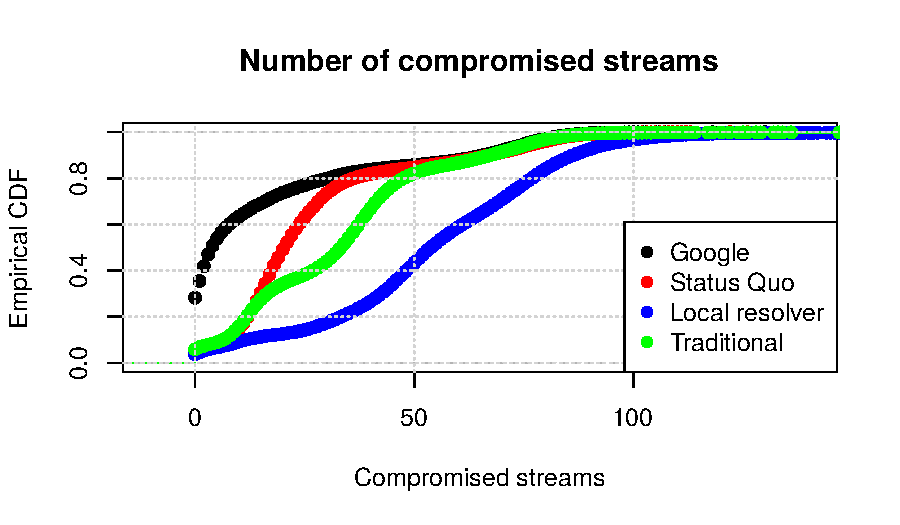
\includegraphics[width=0.6\linewidth]{figures/num-compromised-streams.pdf}
    \label{fig:compromised-streams}
}
\subfigure[Time to first compromise.]{
	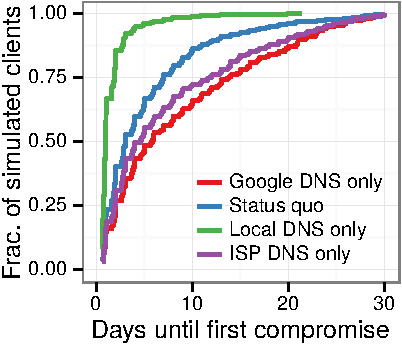
\includegraphics[width=0.6\linewidth]{figures/time-until-compromised.pdf}
    \label{fig:time-until-compromise}
}
\caption{Two emulations for the Tor network in March 2016 show the
  number of compromised streams and the time until the first compromised
  stream.} 
\label{fig:compromise-stream-time}
\end{figure}

Figures~\ref{fig:compromised-streams}
and~\ref{fig:time-until-compromise} show that
Google fared much better than the other situations. This might lead you to believe that 
Tor exit relays should use 8.8.8.8 for all of their name resolution needs, but then you've 
given Google A LOT of power. It might actually be better to tell Tor exit relay operators 
to use their ISPs' default name servers because the ISPs get to see the Tor destinations 
anyway! (Actually, the ISPs fared the best now that we actually measure this
--need to update this paragraph)

The Status Quo results are significantly better than the Local results because only X\% 
of Tor exit relays actually do their own resolution.

Figures for all five of our chosen client ASes will be inserted soon.

